\documentclass[10pt, a4paper]{scrartcl}
\usepackage{amsmath}
\usepackage{amssymb}
\usepackage{graphicx}
\usepackage{subcaption}
\usepackage{float}
\usepackage{geometry}
\usepackage[utf8]{inputenc}
\usepackage{hyperref}
\usepackage[multiple]{footmisc}
\usepackage{parskip}
\usepackage{wrapfig}
\usepackage{xfrac}
\usepackage{xcolor}
\usepackage{tikz}
\usetikzlibrary{arrows}
\usetikzlibrary{arrows.meta}
\usepackage{longtable}
\usepackage{pdfpages}
\usepackage[tikz]{bclogo}

\hypersetup{
    colorlinks=true,
    linkcolor=blue,
    filecolor=magenta,      
    urlcolor=cyan
}

\restylefloat{table}

\newcommand{\warn}[1]{\textbf{#1}}
\newcommand{\con}[1]{\texttt{#1}}
\newcommand{\dis}[1]{\textbf{\texttt{#1}}}

\newenvironment{remember}{\begin{bclogo}[couleur=blue!30,arrondi=.1,logo=\bccrayon,ombre=true]{Remember}}{\end{bclogo}}   
\newenvironment{remark}{\begin{bclogo}[couleur=blue!30,arrondi=.1,logo=\bcinfo,ombre=true]{Remark}}{\end{bclogo}}   
\newenvironment{warning}{\begin{bclogo}[couleur=red!30,arrondi=.1,logo=\bcattention,ombre=true]{Warning}}{\end{bclogo}}   


\title{QRP CW Transceiver Manual}
\subtitle{Board rev. 2, Firmware rev. 2.0}
\author{Hannes Matuschek -- DM3MAT\\\texttt{<dm3mat [at] darc [dot] de>}\\\texttt{https://dm3mat.darc.de/cw2019}}
\date{\today}

\begin{document}
\maketitle
\begin{abstract}
\end{abstract}

\setcounter{tocdepth}{2}
\tableofcontents
\thispagestyle{empty}

\clearpage
\section{Receiver \& Controller Board} \label{sec:rx}
 [TODO RX Description]

\subsection{Controller Assembly}
 In a first step, the controller part of the receiver board is assembled. Install C2, C26, J7, L2, C40, C41, C42, U10, J10, C14, J3, R3, C46, R4, U11 - Socket, LCD1, R43, R5, RV4, J9, R41, R40, C39 \& U9 first. 

\begin{warning}
The metal tab of the TO-220 package of U10 is usually connected directly to the center pin (GND). Please check beforehand if this is the case for your variant. Some rare packages connect this pad to \emph{+5V} leading to a nice \& solid short-circuit that will blow either U10 or L3 or both.
\end{warning}

If you got one of the rare TO-220 variant of U10 that connects the metal tab to +5V, use a mica-insulator between U10 and the PCB.

 R43 limits the current to the LCD backlight. By default a $220\,\Omega$ resistor is installed. This limits the current to about $23\,mA$. This results in a very dim back-light but reduces the current consumption from max. $120\, mA$ (R43 shorted). I personally consider this dim setting the most useful: During daylight a back light makes no sense as the LCD is perfectly readable. During night, without any external light-sources a very dim back light is still sufficient to read the LCD. There is simply no need to drain the battery live for unused or too-bright back lights. If you use the TRX only at home and current consumption is not an issue, you may choose a smaller value for R43 or even bridge it for maximum brightness.
 
\begin{remark} 
 You may also replace the resistor R43 with a push-button at the front panel to switch the back-light on when needed.
\end{remark}
 
 Then, assemble the switch plug and (top right corner labeled \emph{SW}). Connect a 12V power-supply (ideally current-limited to not more than 100mA) to the pads of the supply connector (also top-right corner) labeled \emph{+ G}, where the \emph{+} pad is +12V and the \emph{G} pad is ground. 

\begin{remember}
 The receiver board itself has no reverse-polarity protection. So be careful when connecting the RX board to the power-supply!
\end{remember}
  
 If nothing blows up, switch the TRX off and continue assembling the rotary-encoder and LCD plugs. 
 
 The rotary encoder plug has the following connections (read left-to-right): \emph{Button}, \emph{Encoder B}, \emph{Encoder A}, \emph{Ground}. 

 The LCD-plug has the following connections (read left-to-right): \emph{5V} pin 2 on LCD, \emph{contrast} pin 3 on LCD, \emph{LED backlight} pin 15 on LCD, \emph{GND} pin 1 on LCD, \emph{RS (register selection)} pin 4 on LCD, \emph{D4-D7} pins 11-14 on LCD, \emph{chip-enable (EN)} pin 6 on LCD. You also need to connect pins 5 and 16 on the LCD-board directly to ground (pin 1 on LCD).
 
 Plug the LCD \& rotary encoder into the board and install the ATMega328 MCU. Then connect the board to the power-supply. If you got a pre-programmed MCU you should see a brief greeting on the LCD. If you do not see anything at all or a series of back blocks on the screen, you may have to set the LCD supply/contrast setting using RV4. If you still don't see anything on the LCD, double-check your connects to the LCD! 

\subsection{Testing PLL}
In a next step, verify the SI5351 PLL. First install the SI5351 break-out board. 

\begin{warning}
 Be careful when inserting the SI5351 beakout-board, there is no protection in the socket to plug it in the wrong way: The board should overlap with the LCD connector not U9!
\end{warning}
 
Then switch on the RX and verify that there is a $3.5MHz$ signal at pins 8, 9, 11 and 12 of U9. If not, verify that there is a $14.0Mhz$ signal at the CLK2 output of the SI5351 break-out board. 

You may also verify the $90^\circ$ phase-shift between pins 9 and 12 of U9.

\begin{remark}
By default, the RX is wired to receive on the upper side-band (USB). If you prefer LSB-reception, you may break the jumper labeled \emph{USB} and put a solder-bride on jumper \emph{LSB}. You also need to set the side-band in the firmware.
\end{remark} 

If everything works fine for you so far, continue with assembling the rest of the receiver board.


\subsection{Receiver Assembly}
Before starting to assemble the receiver, disconnect everything from the board. That is, remove the SI5351, LCD and encoder wires and also remove the power-supply wires.

In a first step, install the SMD SOIC-16 FST3253 mixer. 

\paragraph{If you never soldered SMD components before} It is surprisingly simple. Get a sharp soldering-iron tip and thin solder (e.g., $0.75mm$) as well as plenty of flux. Put a lot of flux on the pads. Then put a small amount of solder on one of the pins, for example pin 1 in the bottom-right corner. Pick up the IC with pointy tweezers and place it on the board. Verify the orientation and alignment of the IC. Solder only pin 1 to the board by heating the pad and pushing the IC on the board. Then take a magnifying glass and verify the alignment of all pins with their pads. If needed, reheat pad 1 and improve the alignment. Once the alignment is right, you can start to solder the remaining pads. You do not need much solder! And remember: The flux will do all the work for you. If you got a solder-bridge between two pins, grab some desoldering-wig and remove the solder. 

Once the mixer is installed, the order in which the next components are installed, does not mater. Complete the assembly of the board but leave the board-to-board interconnects (labeled \emph{TX, RX, +G} and the unlabeled 10-pin connector at the bottom) of the board for now. 

\begin{remark}
The audio PA (LM386, U4) has plenty of amplification. If you want to use head-phones, you may leave R13 and C16 off the board. You may add them later if more audio amplification is needed.
\end{remark}

The RCA-Jack J13 is optional. It provides an open-collector output to switch external power-amplifiers. If you plan to use this rig as a pure QRP rig, you may omit that part.

When winding the input transformer T1, cut 3 about 15-16cm long pieces of magnet wire and start the winding by pushing the three wires from the back tough the core. Hold them. Then make the next winding counter-clock wise by pushing the other end of the wires though the core from the front and continue to wind 8 turns on the core counter-clock wise. Every time the wires pass through the core, counts as a turn. 

\begin{remember}
Before soldering the core, make sure the wires are aligned correctly using a multi-meter. That is, top-left connects to bottom left, top-center to bottom-center and top right to bottom right pads on the board. 
\end{remember}

\subsection{Receiver Test and Alignment}
Once the receiver is completed, re-connect the top-right pads \emph{+ G} to the power-supply, prepare the volume and head-phone plug. Also connect a piece of coaxial cable to the \emph{RX/GN} pads in the top-left. This is the antenna input for the test. 

\subsubsection{Frequency Alignment}
If a accurate frequency-counter is at hand, you may start your alignment by fixing the PLL offset. Select the 20m band and tune to $14.0003 MHz$. Then measure the frequency at the USB pad. You should read exactly $14.001 MHz$. If not, enter the Setup menu and select the \emph{PLL correction} option. Now adjust the correction until you read $14.001 MHz$ in the frequency counter.

\subsubsection{Side-band Suppression}
If an signal generator is at hand, tune the generator to $14.000 MHz$. Then select the 20m Band and tune to $14.0012 MHz$. You may hear a low-frequency tone (about $500Hz$). Tune RV2 \& RV 3 to minimize the unwanted side-band tone. Then tune to $14.0016 MHz$. You may hear a high-frequency tone (about $900 Hz$). Tune RV1 \& RV3 to minimize the unwanted side-band tone. You may repeat the previous steps several times to obtain the optimal result. In my experience, the unwanted side-band suppression will work satisfactorily on all bands once aligned properly on 20m. 

With these steps, the alignment of the RX is completed and you may take the RX on a short ride through the bands.


\subsection{RX Component List}  \label{sec:rxcomp}
\begin{longtable}{|l|p{6cm}|l|l|} \hline 
\# & Component & Value & Remarks \\ \hline 
1 & R15 & 10R & \\
4 & R20, R21, R22, R23 & 100R & \\
1 & R43 & 220R & \\
3 & R38, R39, R42 & 1k & \\
1 & R13 & 2.2k & \\
9 & R7, R27, R29-R31, R33, R35-R37 & 3.3k & \\
1 & R32 & 4.3k & \\
1 & R4 & 4.7k & \\
1 & R26 & 5.1k & \\
1 & R34 & 7.5k & \\
10 & R1, R2, R6, R11, R18, R24, R25, R28, R40, R41 & 10k & \\
2 & R9, R10 & 30k & \\
2 & R12, R14 & 33k & \\
2 & R16, R17 & 36k & \\
2 & R3, R5 & 47k & \\
1 & R8 & 120k & \\
1 & R19 & 470k & \\
2 & RV1, RV2 & 50k & \\
1 & RV3 & 500R & \\
1 & RV4 & 10k & \\
3 & C13, C20, C23 & 1n & \\
2 & C25, C27 & 3.3n & \\
3 & C30, C31, C35 & 10n & \\
5 & C12, C17, C18, C21, C33 & 47n & \\
23 & C3, C8, C11, C22, C24, C26, C29, C32, C34, C37-C41, C46-C54 & 100n & \\
5 & C4, C5, C6, C7, C36 & 470n & \\
2 & C1, C28 & 1u & \\
3 & C15, C16, C42 & 10u & \\
3 & C2, C14, C19 & 100u & \\
6 & L1, L3, L4, L5, L6, L7, L8, L9 & 100u & \\
1 & T1 & 3 x 8 @ FT37-43 & \\
1 & D1 & 1N4148 & \\
1 & Q1 & BS170 & \\
1 & Q2 & 2N3904 & \\
1 & U1 & FST3253 & \\
5 & U3, U5, U6, U7, U8 & LM833 & \\
1 & U4 & LM386 & \\ 
6 & -- & DIP-8 Sockets & \\
1 & U9 & 74AC74 & \\
1 & U10 & L7805 & \\
1 & U11 & ATmega328-PU & \\
1 & --  & DIP-28 Socket & \\
1 & - & SI5351 break-out & \\
2 & J1, J3, J4, J11 & 1x10 pin-header long & \\
1 & J6 & 2x3 pin-header & \\
1 & J9 & 1x7 pin-socket & \\
2 & J2, J7 & 1x2 90deg & \\
1 & -- & Switch & \\
1 & J8 & 1x3 90deg & \\
1 & -- & 10k log & potentiometer \\
1 & J10 & 1x4 90deg & \\
1 & -- & Rotary encoder & \\
1 & LCD1 & 1x8 90deg & \\
1 & -- & LCD & 2 x 8 symbols \\
1 & J13 & TX-OC & RCA-jack (optional) \\
1 & J5 & Key & 3.5mm stereo jack\\ \hline
\end{longtable}

\clearpage
\section{PA \& Low-Pass Board} \label{sec:pa}
The majority of the PA/LP board consists of 4 7-pole Chebyshev low-pass filters. The Chebyshev-type filters are needed to get away with only 4 filters to cover all RF band from 80m-10m. The right-most filter covers the 80m and 60m band and should have a cut-off frequency near $5.6\,MHz$. The next filter covers 40m and 30m and should have a cut-off frequency near $10.5\,MHz$. The second-to-last filter covers 20m and 17m and should have a cut-off frequency near $20\,MHz$. Finally the left-most filter will cover 15m, 12m and 10m with a cut-off frequency near $30\,.MHz$. The low-pass filters are switched by 4 sub-miniature relays controlled by the RX-board via board-to-board J2.

The Q4 mosfet acts as the TX/RX switch passing the LP-filtered RF from the input to the RX via J6.

The PA section consist of a 74HCT00 as a pre-driver, 4 BS170 mosfets as PA Transistors and a BD140 for key-shaping. The TX oscillator signal arrived from the RX-board via J7.

The complete TRX is powered from the barrel-jack J3 and the supply voltage is passed to the RX-board via J11. 

\begin{remark}
 Before assembling the low-pass filers on the board. Please assemble them ugly-style on a piece of PCB material and measure their properties using a network analyzer or spectrum analyzer. Being Chebyshev low-pass filter, the exact component values are critical!
\end{remark}

 If no measurement equipment is present. Please subtract one winding from the given values below. The number of turns for each core was determined using the AL-value provided by the manufacturer. In my experience, this leads to an slightly overestimation of the number of turns by about one. Moreover, you are probably more willing to risk a lower stop-band suppression rather than an increased damping in the pass band.
 
 The diode D4 is connected in parallel to the barrel-jack and acts together with a fuse as a reverse-polarity protection. If the supply is connected to the TRX in reverse-polarity, the diode will short the input which will cause a huge current that blows the fuse. A 2A \emph{flink} or 1A \emph{träge} fuse will do.
 
\subsection{PA/LP Component List}  \label{sec:pacomp}
\begin{longtable}{|l|p{6cm}|l|l|} \hline 
\# & Component & Value & Remarks \\ \hline 
2 & R12, R13 & 100 & \\
1 & R9 & 470R & \\
1 & R10 & 1k & \\
1 & R14 & 4.7k & \\
7 & R1, R3, R5, R7, R11, R15, R16 & 10k & \\
4 & R2, R4, R6, R8 & 100k & \\
2 & C2, C15 & 100p & NP0 \\
4 & C3, C6, C11, C16 & 220p & NP0 \\
4 & C4, C7, C12, C17 & 470p & NP0 \\
2 & C5, C18 & 820p & NP0 \\
2 & C8, C13 & 1n & NP0 \\
2 & C9, C14 & 1.5n & NP0 \\
11 & C1, C10, C19, C20, C22, C23, C24, C27, C28, C29, C30 & 100n & \\
1 & C25 & 1u & \\
1 & C26 & 220u & \\
1 & L13 & 100u & MICC \\
3 & L1, L5, L9 & 330n & 11T on T37-6 \\
3 & L2, L6, L10 & 480n & 13T on T37-6 \\
3 & L3, L7, L11 & 750n & 14T on T37-2 \\
3 & L4, L8, L12 & 1700n & 21T on T37-2 \\
1 & T1 & -- & 8T + 8T on FT37-43 \\
4 & K1, K2, K3, K4 & G6S-2 & \\
4 & D1, D2, D3, D5 & 1N4148 & \\
1 & D4 & 1N4001 & \\	
4 & Q1, Q2, Q3, Q10 & 2N3904 & \\
6 & Q4, Q6, Q7, Q8, Q9, Q11 & BS170 & \\
1 & Q5 & BD140 & \\
1 & U1 & 74HCT00 & \\
1 & J1 & BNC & \\
1 & J2 & 1 x 8 pin-socket & \\
1 & J3 & barrel-jack & \\
3 & J6, J7, J11 & 1 x 2 pin-socket & \\ \hline
\end{longtable}


\clearpage
\section{Final Assembly} \label{sec:box}
Finally, the board-to-board interconnects are installed. The way these connectors are installed, depends on the chassis you chose and the distance between the boards. The example I give here applies to the Fischer KOH-2100 + KOH-4100 kit. This is a nice compact $10 \times 10 \times 5\,cm$ chassis. The boards slide into the chassis with $2.03\,cm$ distance. Unfortunately, I was not able to find stackers or long pin-headers with a matching length here in Germany. Have a look at Ebay or at Mouser, pin headers with insertion lengths of about 18mm should do the trick. Maybe you are lucky.

I went with stackers of 38mm total length which is is to long.

\subsection{Final Testing}
With these stacked boards, it is now time to test the PA and RX/TX switching. Connect a dummy-load to the output and measure the RF voltage-drop across the dummy-load. Alternatively, connect a power/SWR meter between the TRX and dummy-load. You should get about $22\,Vp$ across the dummy-load or about 5W on transmit depending on the supply voltage (assuming about $13.8\,V$). On the lower band (e.g., up to 30m) it might even be a little bit more. 

If your output is way less, measure the peak voltages at the PA-output and LP-input and double-check the low-pass filters. If the output matches, the assembly is complete. 

\clearpage
\section{Usage} \label{sec:user}
Handling a feature-rich TRX using a single rotary encoder with a single push-button is kind of challenging. I've designed a two-level menu navigation that puts everything, that is needed frequently, in the first level (blue in figure \ref{fig:menu}) and everything else in a second level. This keeps the navigation fast for frequently used options. 

The second menu level (red in figure \ref{fig:menu}) contains all settings that are usually not touched during the operation. They concern the basic setup and alignment of the TRX. 

\begin{figure}[!ht]
 \centering
 \footnotesize
 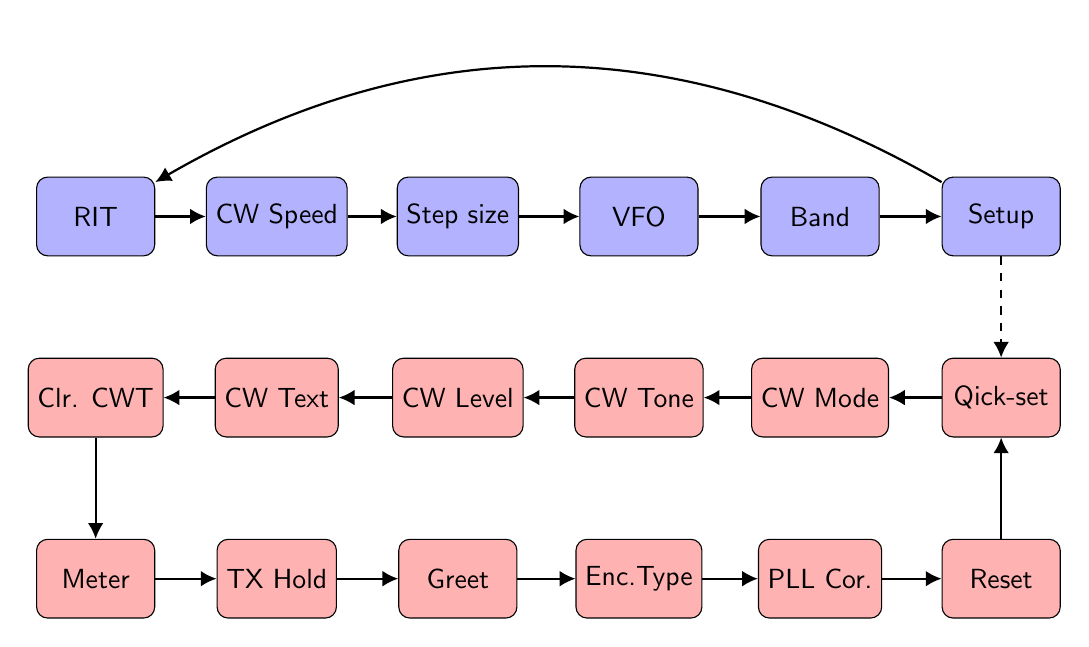
\begin{tikzpicture}[node distance=2.3cm,
	>={Latex[width=2mm,length=2mm]},
    menu/.style = {rectangle, rounded corners, draw=black,
                   minimum width=1.5cm, minimum height=1cm,
                   text centered, font=\sffamily, fill=blue!30},
    submenu/.style = {menu, fill=red!30}]
  \node (rit) [menu] {RIT};   
  \node (speed) [menu, right of=rit] {CW Speed}; 
  \node (step) [menu, right of=speed]{Step size};
  \node (vfo) [menu, right of=step] {VFO};
  \node (band) [menu, right of=vfo] {Band};
  \node (setup) [menu, right of=band] {Setup};
  
  \node (quick) [submenu, below of=setup] {Qick-set};
  \node (cw) [submenu, left of=quick] {CW Mode}; 
  \node (tone) [submenu, left of=cw] {CW Tone}; 
  \node (level) [submenu, left of=tone] {CW Level}; 
  \node (text) [submenu, left of=level] {CW Text}; 
  \node (clr) [submenu, left of=text] {Clr. CWT};
  \node (meter) [submenu, below of=clr] {Meter};
  \node (hold) [submenu, right of=meter] {TX Hold}; 
  \node (greet) [submenu, right of=hold] {Greet};
  \node (enc) [submenu, right of=greet] {Enc.Type};
  \node (pll) [submenu, right of=enc] {PLL Cor.};
  \node (reset) [submenu, right of=pll] {Reset};
  
  
  \path[->,thick]
    (rit) edge (speed)
    (speed) edge (step)
	(step) edge (vfo)
	(vfo) edge (band)
	(band) edge (setup)
	(setup) edge[bend right] (rit);
	
  \path[->,thick,dashed]
    (setup) edge (quick);
  \path[->,thick]
        (quick) edge (cw)
    	(cw) edge (tone)
    	(tone) edge (level) 
    	(level) edge (text)
    	(text) edge (clr)
    	(clr) edge (meter) 
    	(meter) edge (hold)
    	(hold) edge (greet) 
    	(greet) edge (enc)
    	(enc) edge (pll)
    	(pll) edge (reset) 
    	(reset) edge (quick);
 \end{tikzpicture}
 \caption{Menu navigation} \label{fig:menu}
\end{figure}

To enter the menu, just click the center button on the rotary encoder. You will land on either the RIT setting or on the last modified setting. Using the rotary-encoder you can navigate through the first menu level. To change a settings, click the center button again. You can now change the selected setting using the rotary encoder. To finish the setting and leave the menu, click on the center button again.

To enter the second menu-level, enter the first level by clicking on the center button and select the menu entry \texttt{Setup}. Click on the center button again to enter the second-level menu. You will land on the \texttt{Quick-set} setting. You may now navigate the second menu-level using the rotary encoder. Changing and leaving the second-level menu works in the same way as the first-level menu. 

\paragraph{Receive/Transmit offset (RIT)}
[TODO]

\paragraph{CW speed}
[TODO]

\paragraph{Tuning step-size}
[TODO]

\paragraph{VFO}
[TODO]

\paragraph{Band}
[TODO]

\paragraph{Setup}
[TODO]

\paragraph{Quick-set}
(Planned Feature) The Quick-set feature allows to set a specific property without entering the menu. By holding and turning the rotary-encoder at the same time. This menu item allows to select one of four settings to be manipulated by the quick-set feature: RIT, keyer speed, tuning step-size, band or \emph{none}. The latter disables the quick-set feature.

\paragraph{Keyer mode}
[TODO] Straight Key, Iambic, (planned) Iambic reverse, (planned) auto detect

\paragraph{CW side-tone frequency}
[TODO]

\paragraph{CW side-tone level}
[TODO]

\paragraph{Keyer memory}
[TODO]

\paragraph{Clear keyer memory}
[TODO]

\paragraph{Meter selection}
[TODO]

\paragraph{TX-hold time}
[TODO]

\paragraph{Greet text}
[TODO]

\paragraph{Encoder type}
[TODO]

\paragraph{PLL correction}
[TODO]

\paragraph{Factory reset}
[TODO]





\clearpage
\section{Bill-of-Material (BOM)}
\begin{longtable}{|p{0.05\textwidth}|p{0.2\textwidth}|p{0.44\textwidth}|p{0.07\textwidth}|p{0.07\textwidth}|}\hline
\end{longtable}

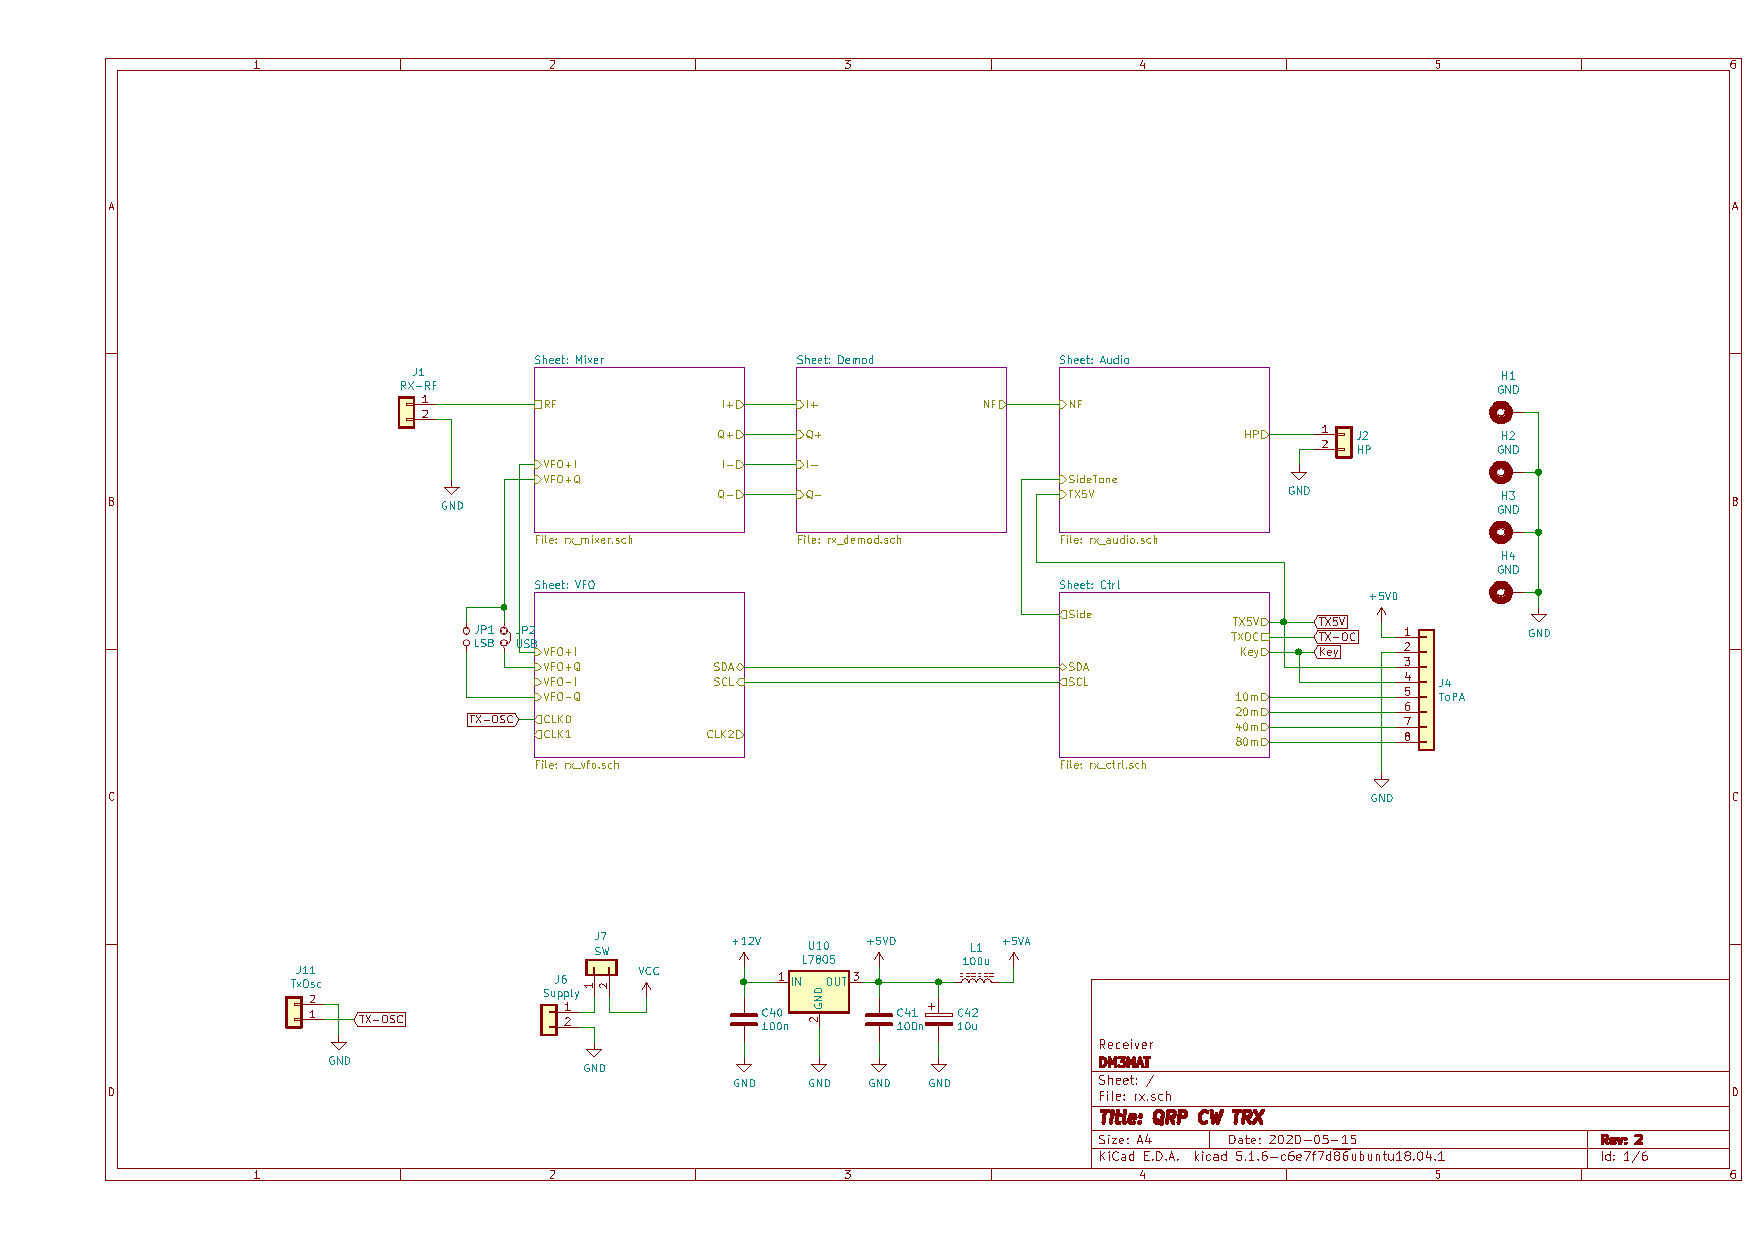
\includepdf[pages={1,2,4,3,5,6},landscape=true, addtotoc={
 1, section, 1, RX Circuit, rxscm,
 2, subsection, 1, RX Mixer, rxmix,
 4, subsection, 1, Demodulator, rxdemod,
 3, subsection, 1, AF-Section, rxaudio,
 5, subsection, 1, PLL, rxpll,
 6, subsection, 1, Controller, rxctrl}]{fig/rx_scm.pdf}
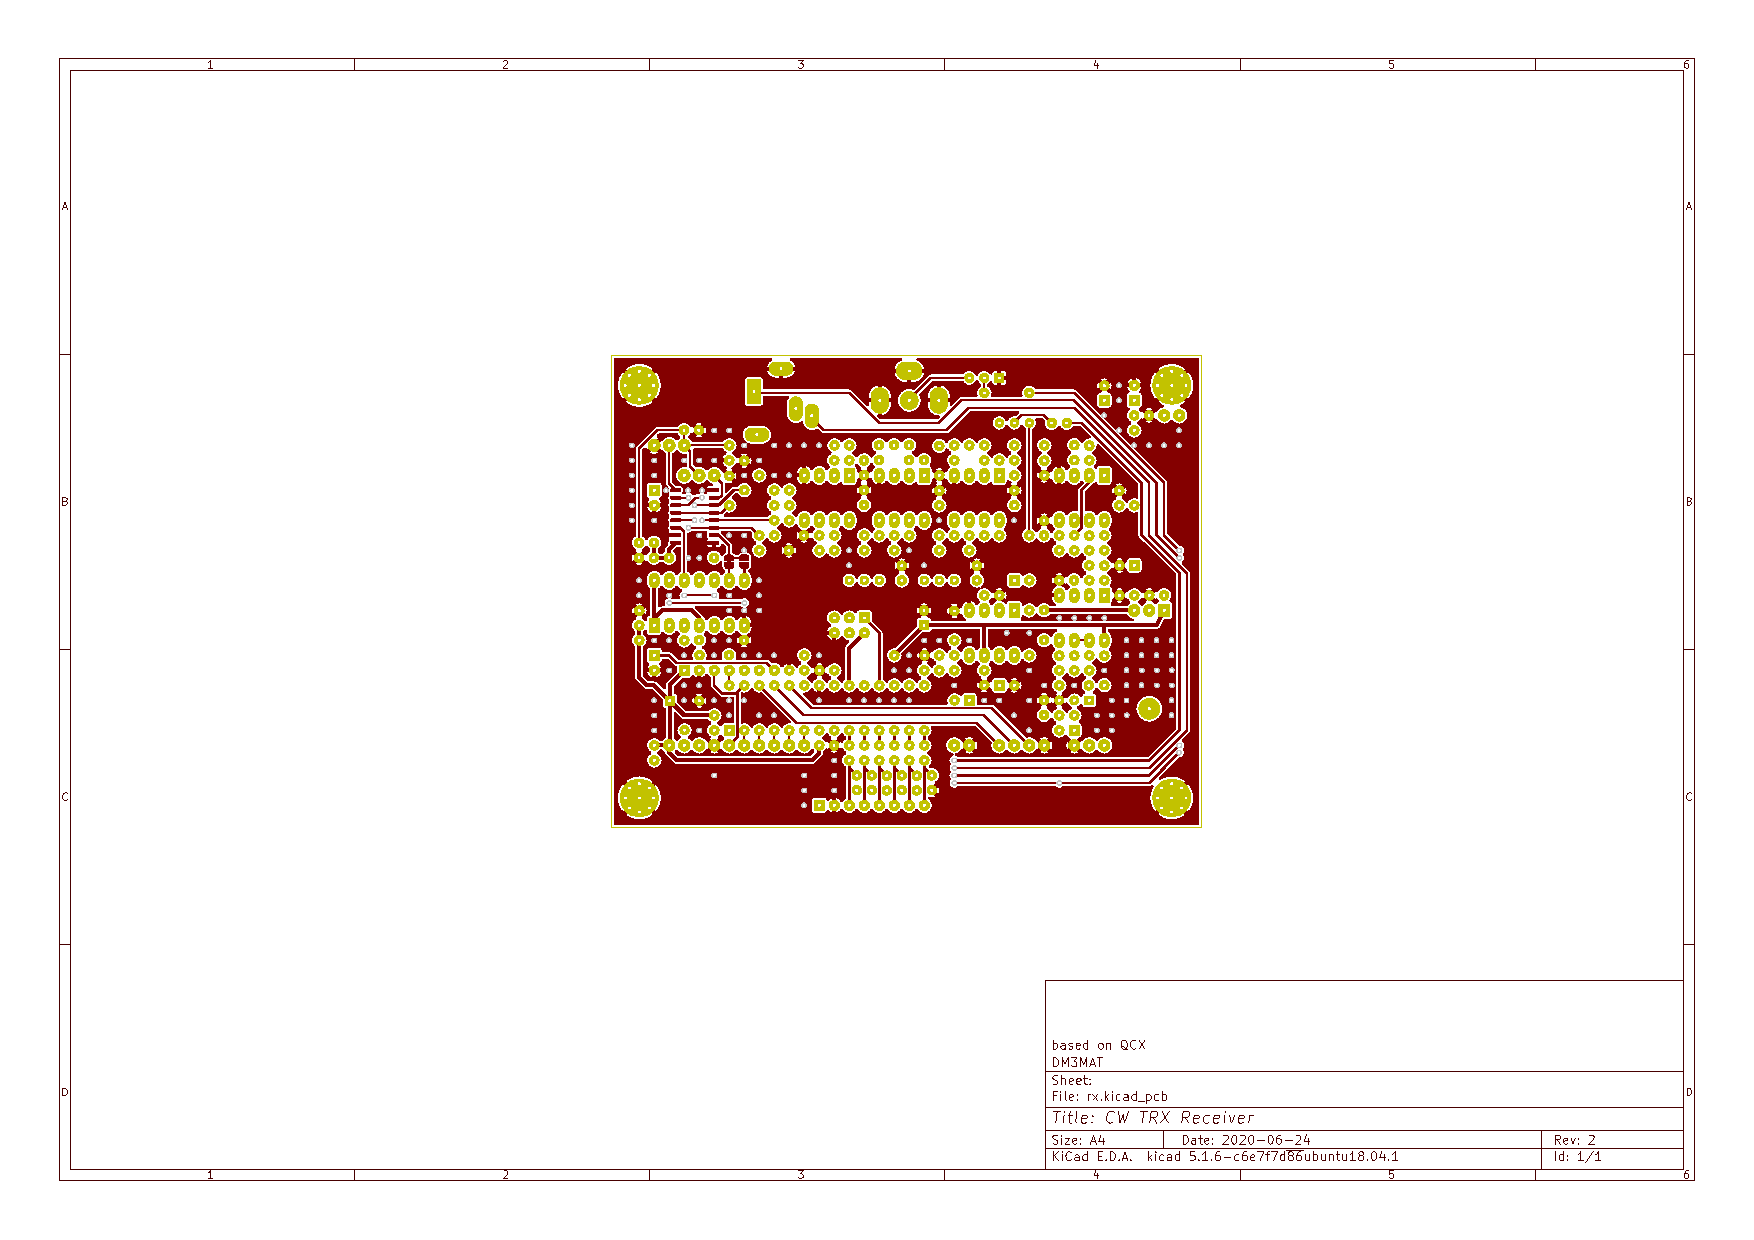
\includepdf[pages={1,2,3},landscape=true, addtotoc={
 1, section, 1, RX Board, rxbrd}]{fig/rx_brd.pdf}
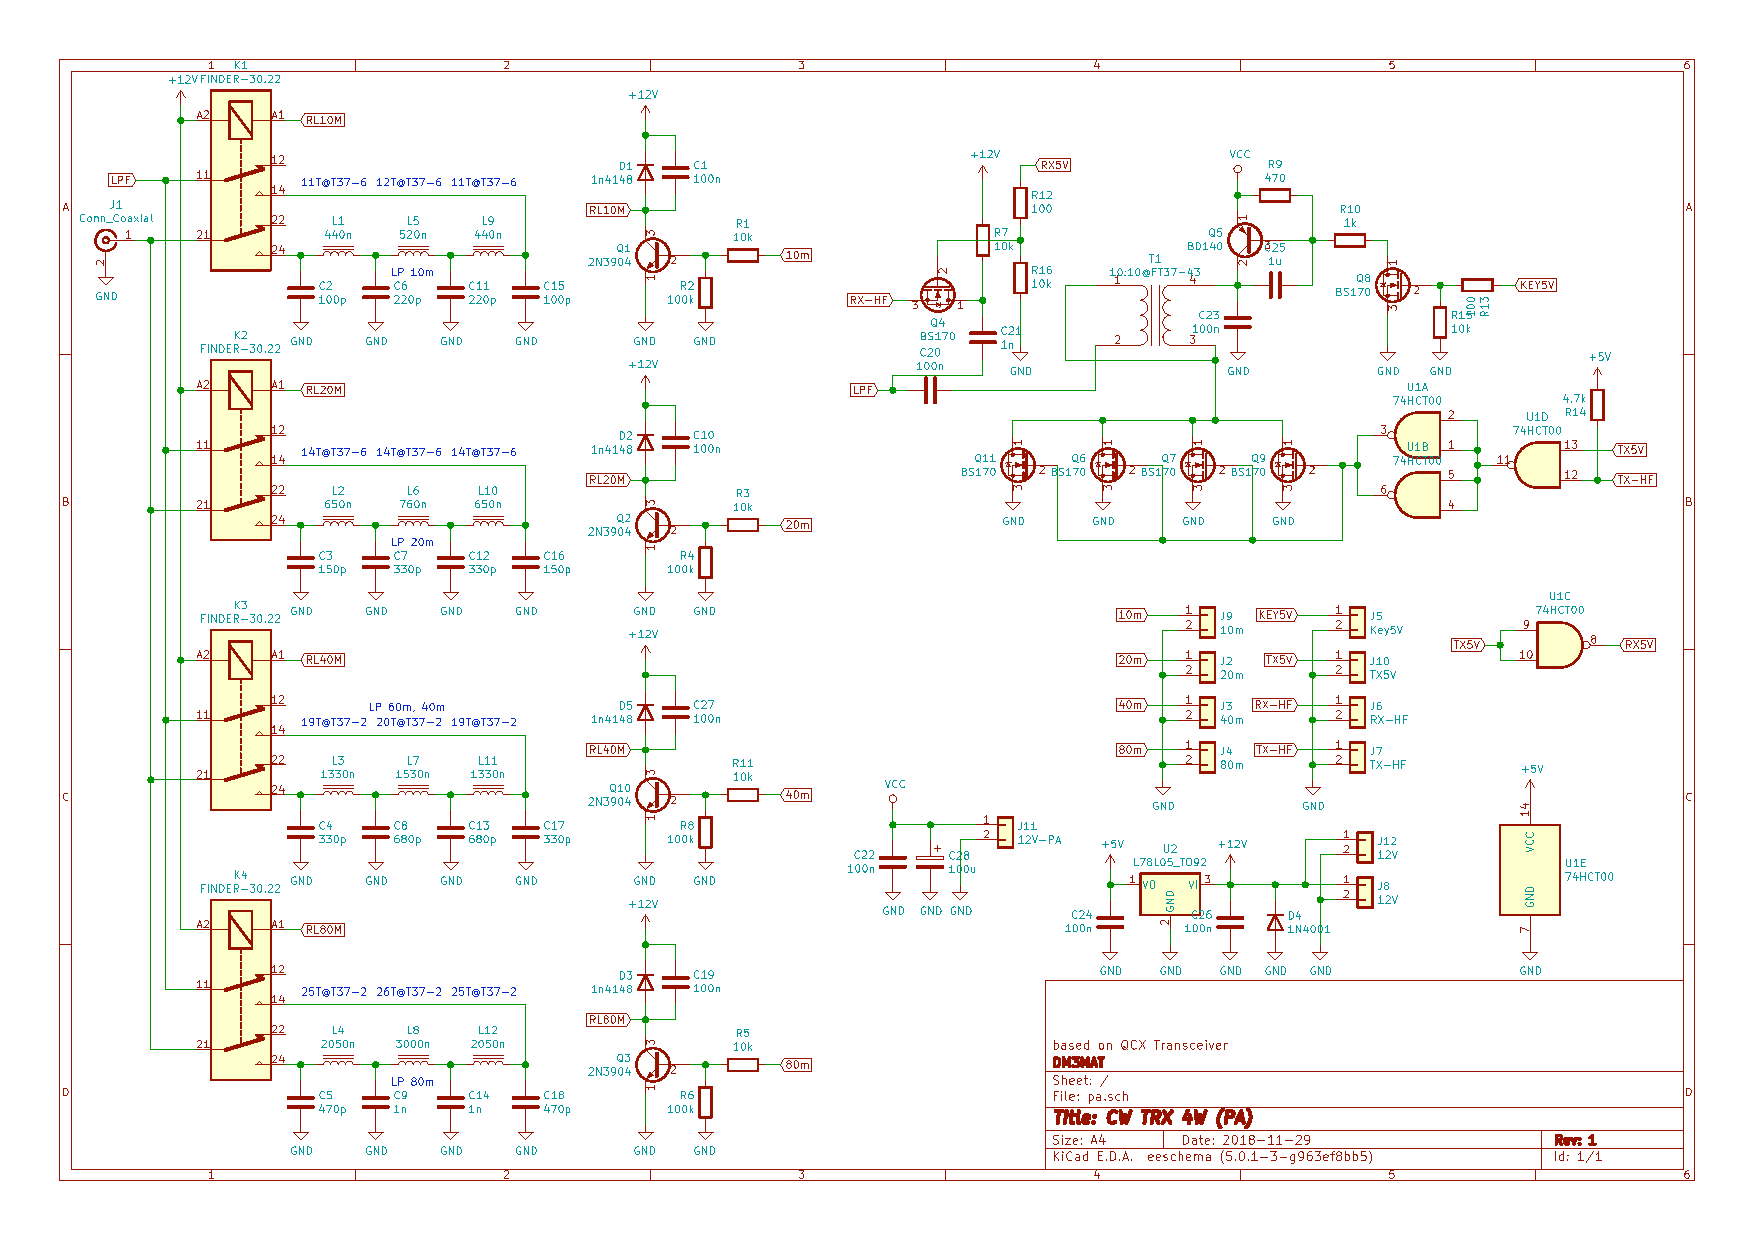
\includepdf[landscape=true, addtotoc={
 1, section, 1, PA/LP Circuit, pascm}]{fig/pa_scm.pdf}
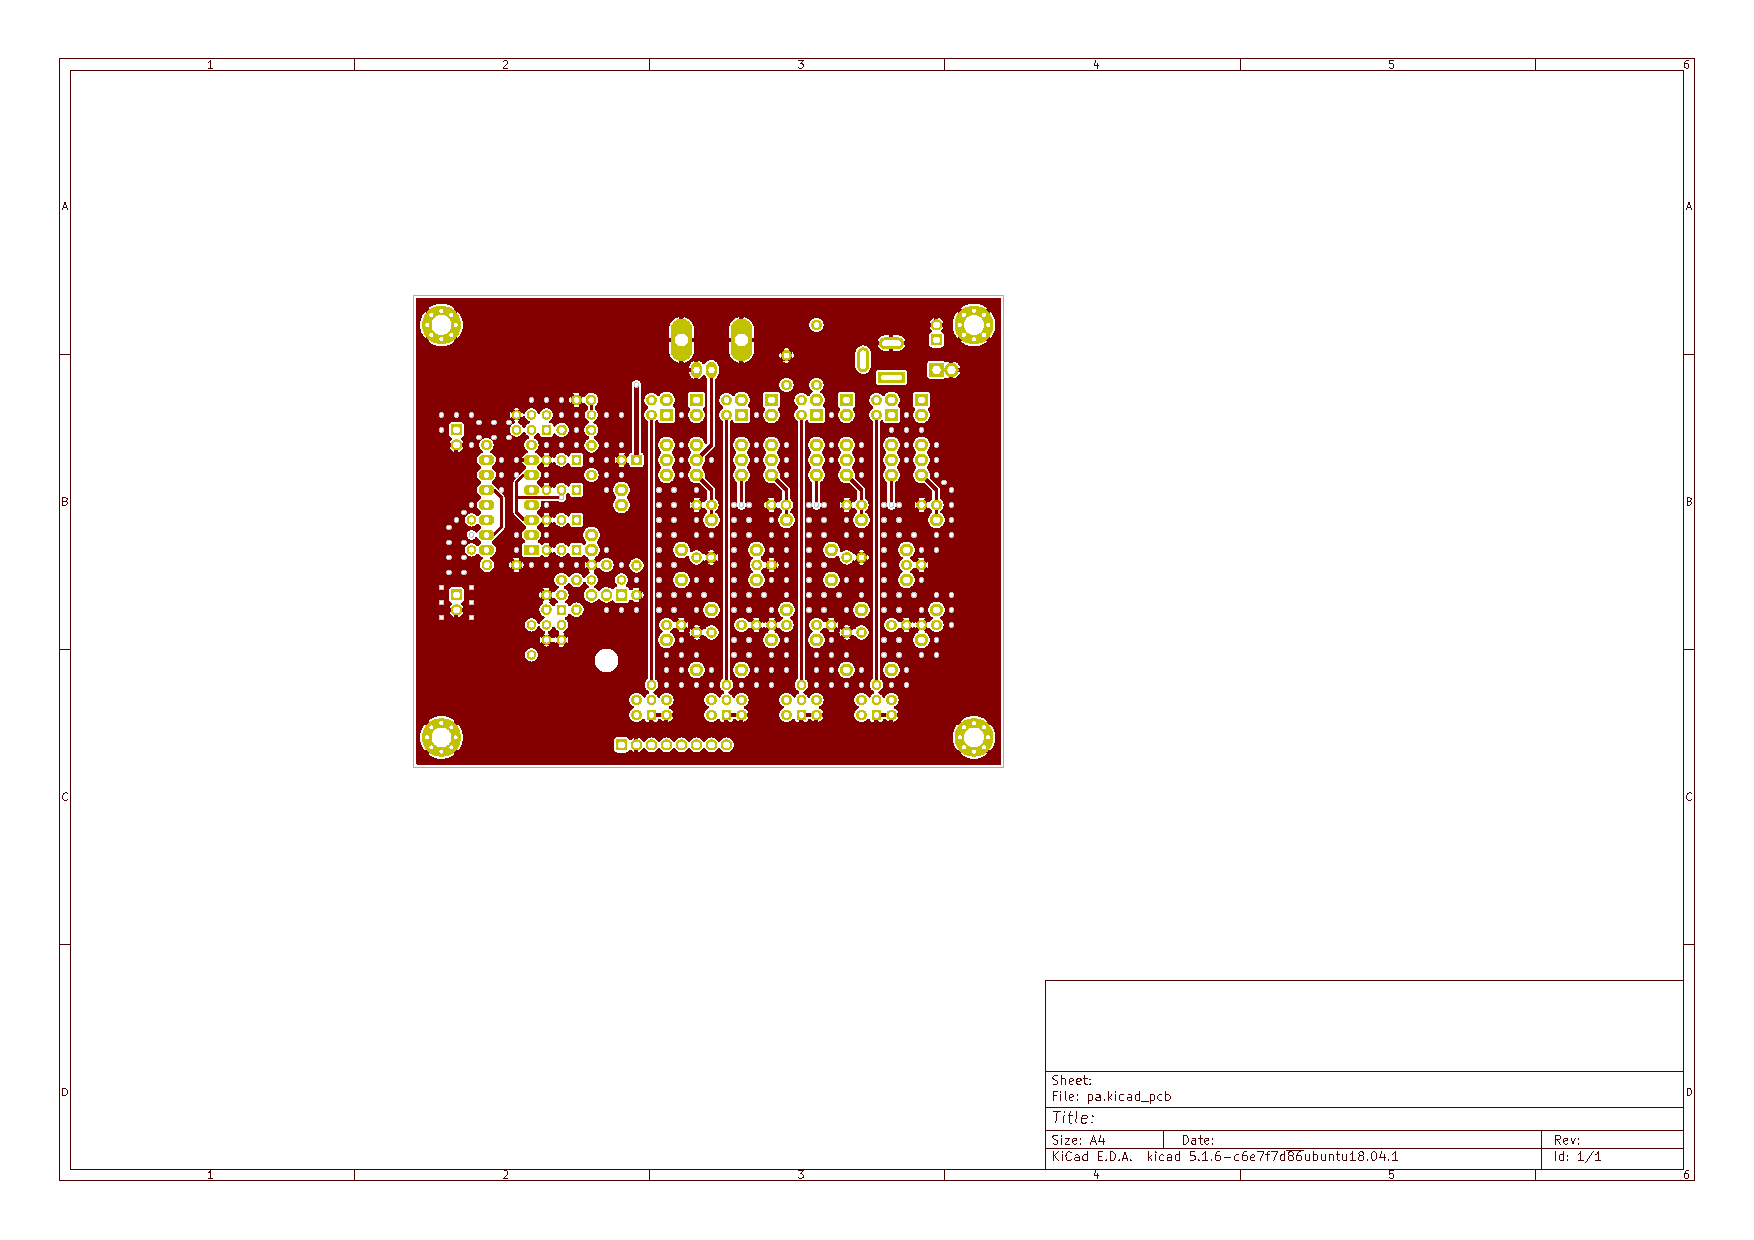
\includepdf[pages={1,2,3},landscape=true, addtotoc={
 1, section, 1, PA/LP Board, pabrd}]{fig/pa_brd.pdf}
\end{document}